\subsubsection{Unfolding}
%The general idea behind the  unfolding operation 
%\begin{align*}
%\ranked{
%    \unfoldsmall : \shallowterm {(\reduce k   \Sigma)} {\Gamma^k} \to \reduce 1 (\shallowterm \Sigma \Gamma)
%}
%\end{align*} 
%is to eliminate a $k$-fold by matching it with a $k$-th power. 
%The unfolding operation is explained in the following picture for $k=2$: 
%        \begin{center}
%        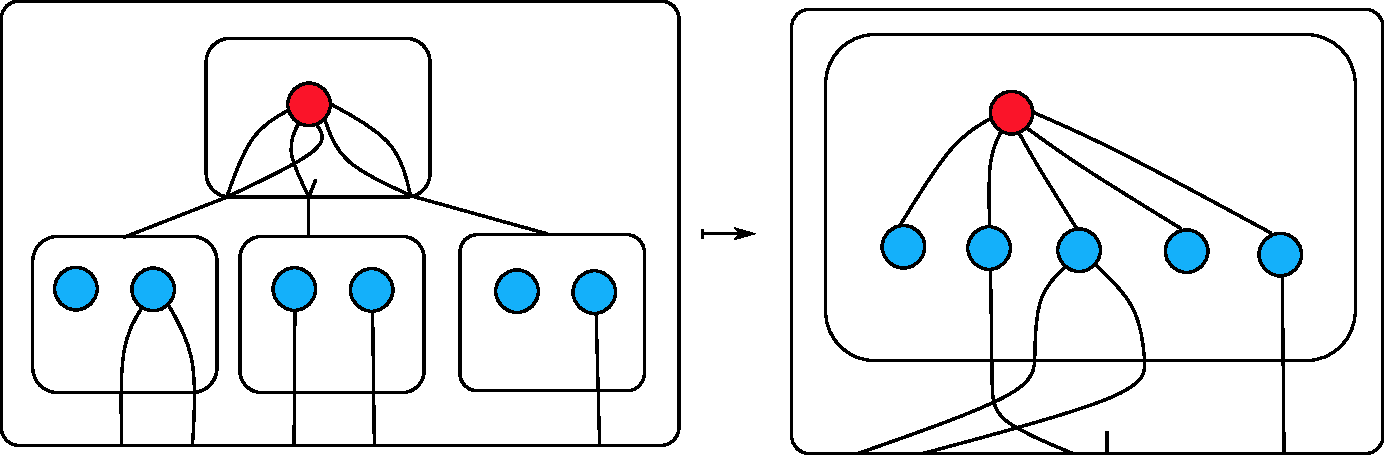
\includegraphics[scale=.36]{shallow-unfold.pdf}
%        \end{center}

In this section, we define the matrix power, which can be seen as a way of representing several trees in one. %Roughly speaking, the several trees are the contents of registers in a register automaton.
%, and the single tree that represents them is the computation tree of the register automaton.  We then show that several trees stored in a computation  can be unfolded in a derivable way. 

\begin{definition}
    [Matrix power] For $k \in \set{1,2,\ldots}$ define the $k$-th matrix power\footnote{
        The name  matrix power is based the matrix power in  universal algebra (for the latter, see~\cite{Taylor1975} or~\cite{szendrei1990simple}). Roughly speaking, the restrictions that we place on the original definition correspond to the single-use and monotone conditions from Definition~\ref{def:stt}. 
     } of a ranked set $\rSigma$ 
to be 
\begin{align*}
 \mati k \rSigma \quad \eqdef \quad \ranked{\reduce k \rSigma^k}.
\end{align*}
\end{definition}

Here is a picture of a binary element in the matrix power, where $k=3$:
\begin{center}
\includegraphics[scale=.4, page=85]{pics.pdf}
\end{center}

, this operation of determining the dependency tree is what we call \emph{unfolding}. We illustrate it by the following example 
\begin{center}
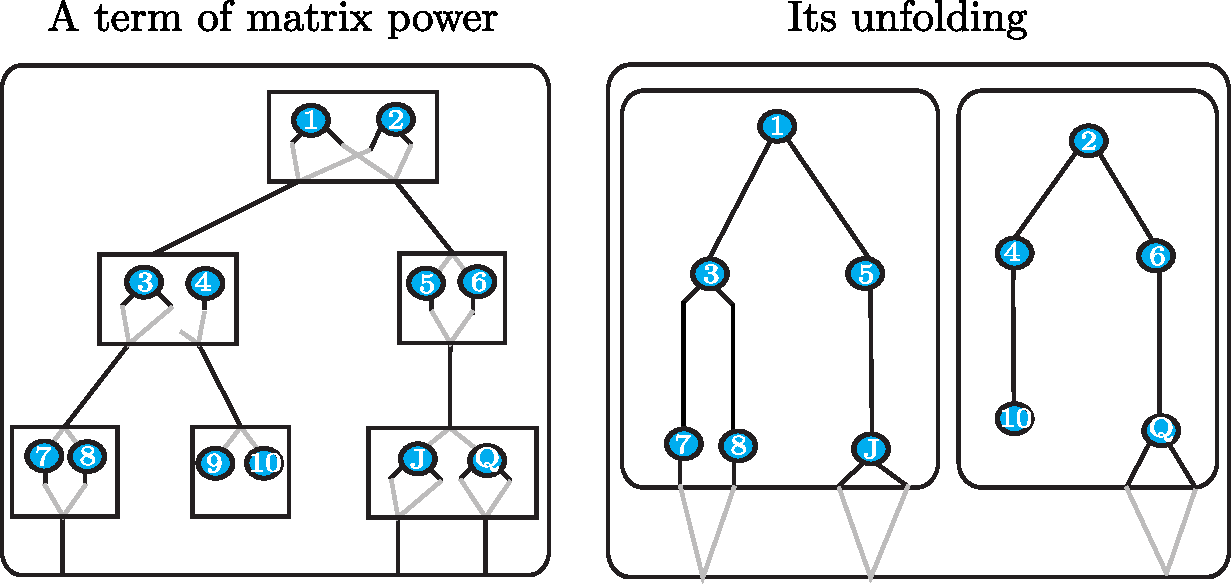
\includegraphics[scale=.38]{unfold-matrix-power}
\end{center}
Formally, \emph{unfolding} is a function of type
\begin{align*}
    \ranked{\unfold : \tmonad \mati k \rSigma \to \mati k {(\tmonad \Sigma)} }
    \end{align*}
 which is defined as follows by induction on the size of the input term. If the input is an empty term, then the output is this term:
\begin{center}
\includegraphics[scale=.3, page=83]{pics.pdf}
\end{center}
Otherwise, if the input is a nonempty term $a(t_1,\ldots,t_n)$ then the output is obtained by first applying unfolding to to the smaller terms $t_1,\ldots,t_n$, and then applying the following derivable function, which we call \emph{shallow unfold}. 
\begin{align*}
    \ranked{
        \xymatrix{
            \shallowterm{\mati k \rSigma} {\mati k \rGamma}  \ar[r] & \mati k {(\shallowterm \Sigma \Gamma)}.
        }
    }
\end{align*}
Here is a picture of unfolding for shallow terms:
\begin{center}
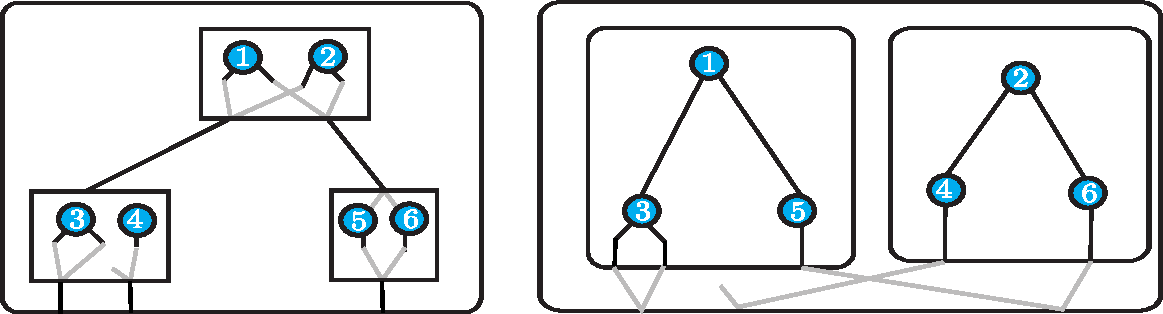
\includegraphics[scale=.4]{unfold-shallow}
\end{center}